\myChapter{Contribution to Machine Learning-Based Anomaly Detection for DNS Transactions}{}\label{chapFusionConsens}
%\myMinitoc{Profondeur de la minitoc (section|subsection|subsubsection)}{Titre de la minitoc}
\myMiniToc{}{Contents}
%\mySectionStar{Titre}{Titre court}{Ajouter à la table des matières? (false|true|chapter|section|subsection|subsubsection -section par défaut-)}
\mySection{Introduction}{}


This chapter unfolds our contributions towards refining DNS traffic analysis by transitioning from traditional binary classification to a more sophisticated multi-class classification framework. Our methodology leverages detailed preprocessing of DNS data, coupled with an in-depth feature engineering process that utilizes correlation analysis to select and transform the most impactful features. We further enhance the classification model by employing advanced clustering techniques, such as DBSCAN, to identify and define new class labels that correspond to distinct categories of DNS-based threats. These methodological advancements enable our models to capture a broader spectrum of malicious activities, offering a more granular and actionable insight into DNS traffic. The implementation of these techniques not only boosts the detection accuracy but also paves the way for deploying these models in practical cybersecurity settings. By providing a detailed account of these processes, this chapter aims to demonstrate how our innovative approach can significantly improve the effectiveness of cybersecurity measures, thereby fortifying network defenses against an array of DNS threats.




\mySection{Contribution To Binary Classification}{}
\subsection{datasets and description}
The CIC Bell DNS EXF 2021 dataset \cite{CIC_Bell_DNS_EXF_2021} is a comprehensive dataset designed to enhance research in the field of network security. This dataset contains detailed records of network traffic with a focus on DNS (Domain Name System) traffic. The dataset is structured to include both benign and attack traffic, with the intention of facilitating the development and evaluation of security solutions such as intrusion detection systems (IDS) and anomaly detection algorithms.The dataset is typically provided in CSV format.
Each file contains multiple records, each representing a single network packet or flow.The dataset includes both stateful and stateless features, capturing various aspects of the network traffic. It contains four classes: heavy attacks,light attacks,heavy benigns and light benigns. It has 756 columns of 148 integers,162 strings,108 decimals and 18 others.It has a size of 270.8MB.It incorporates 42 features, extracted from the DNS packets, ranging to approximately 1,019,318 samples. Out of these 42 features, 15 are stateless, 26 are stateful,and timestamp feature. Stateless features, extracted from individual DNS query packets, are independent of the temporal characteristics of queried domains or the DNS activity of hosts, thus minimizing computational strain during real-time operations. In contrast, stateful features consider a sequence of queries within a specific time window,imposing a greater computational burden on the detection system. However,for binary classification purposes, these four classes are grouped into two broader categories:\\
Attack (1): This includes both heavy and light attack traffic.\\
Benign (0): This includes both heavy and light benign traffic.\\



\newpage
\subsection{model architecture and description}


\begin{figure}[ht!]
    \centering
    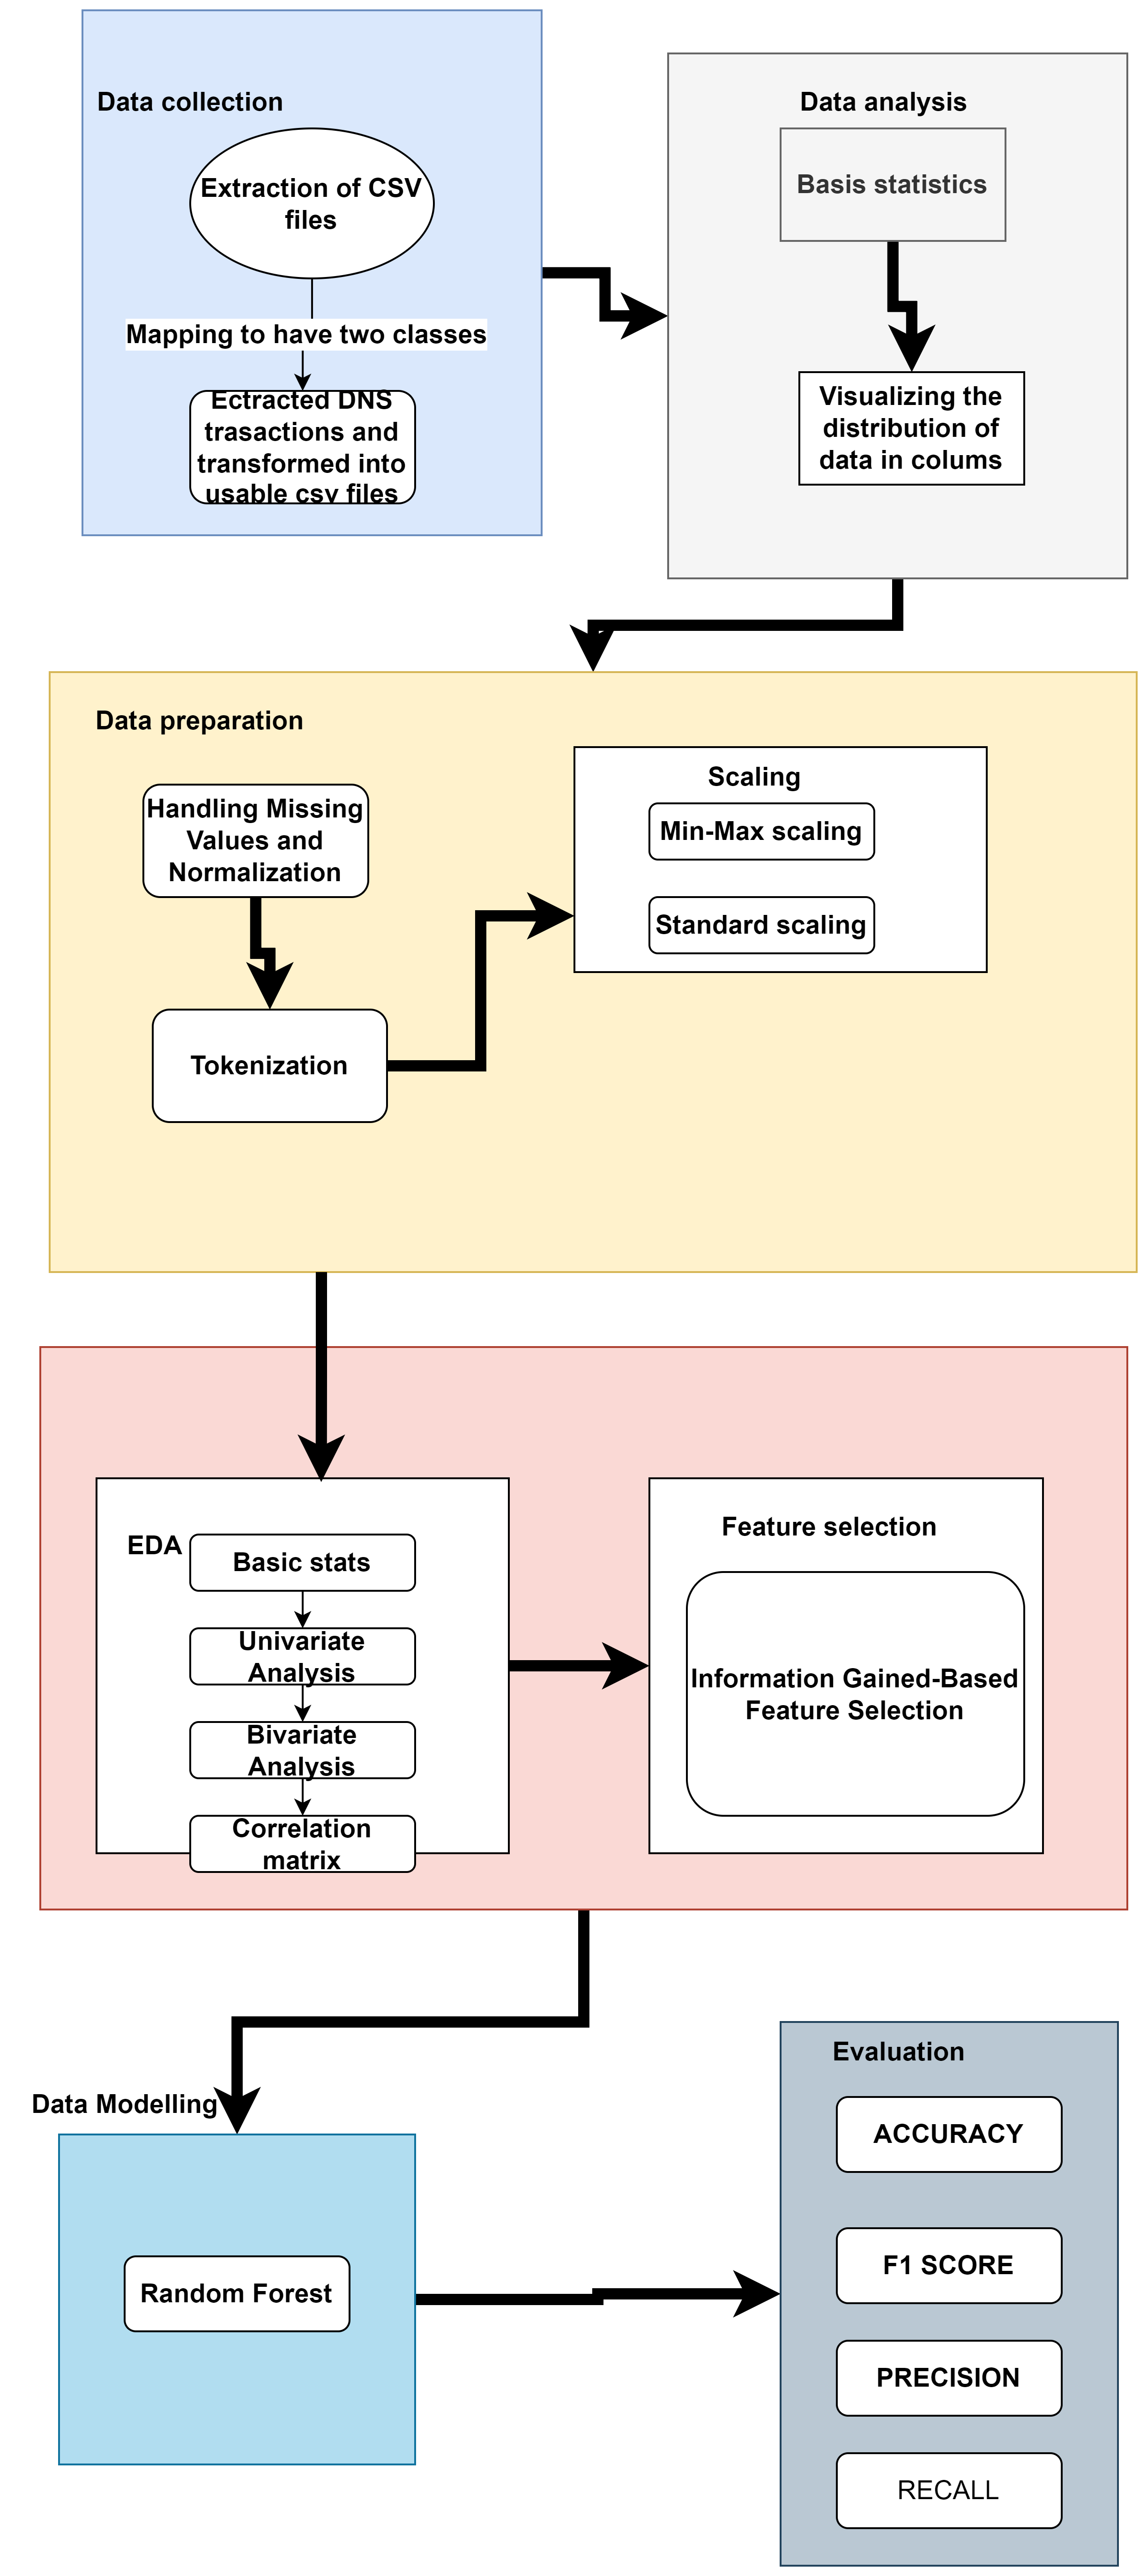
\includegraphics[width=0.6\linewidth]{chap3/images/Architecture binary Diagram2.drawio.png}
    \caption{Proposed binary architecture}
    \label{fig:enter-label}
\end{figure}




\begin{figure}
    \centering
    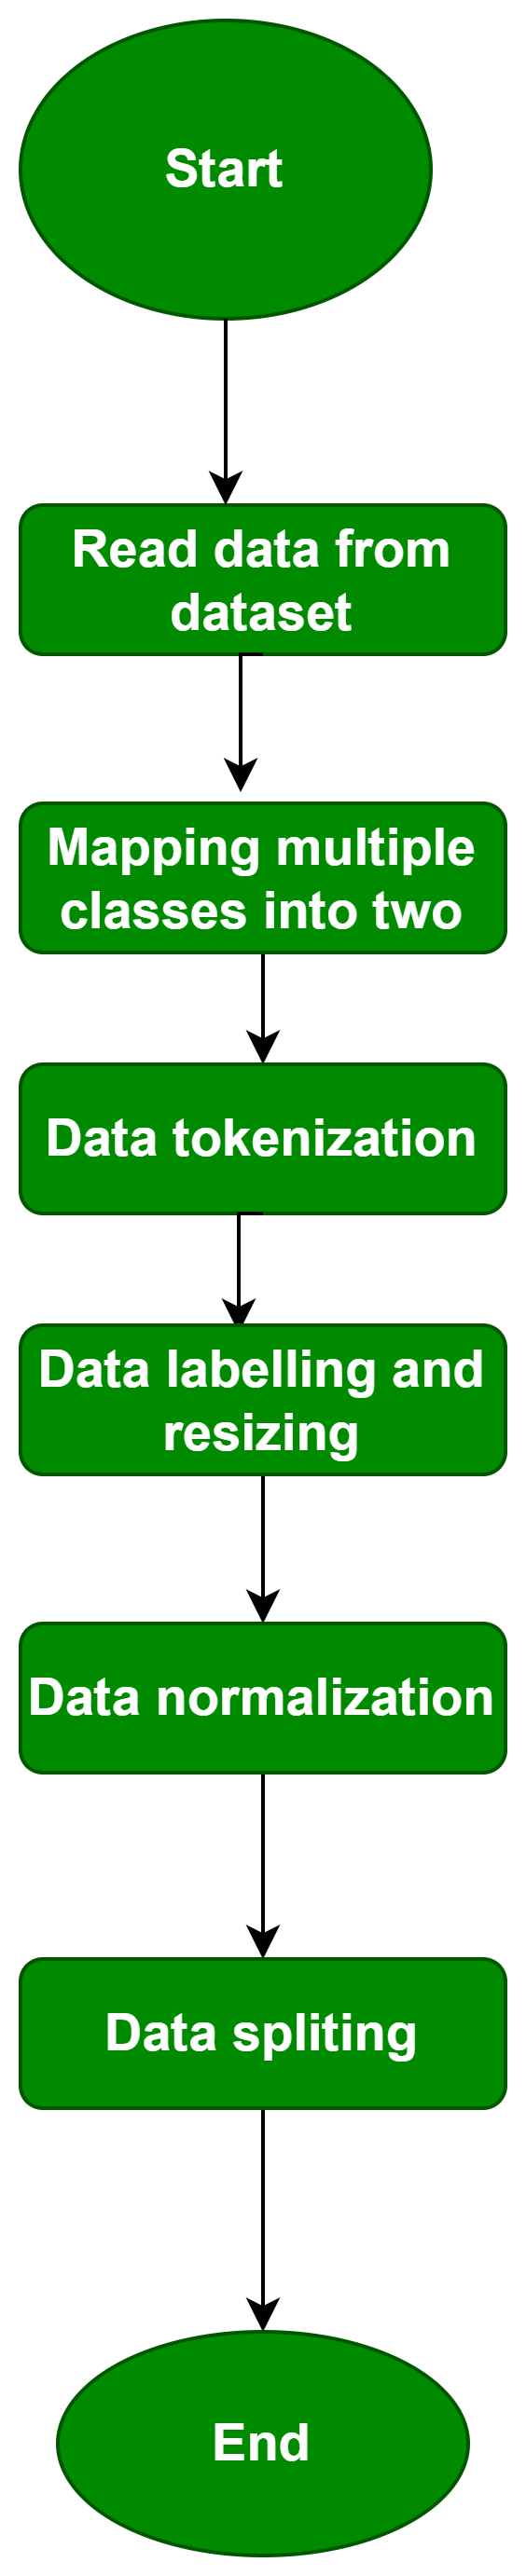
\includegraphics[width=0.3\linewidth]{chap3/images/datapreprocessing binary.drawio.png}
    \caption{ Binary data preprocessing}
    \label{fig:enter-label}
\end{figure}


\newpage


\subsection{Architecture description and preprocessing}
\subsubsection{Read data from dataset}
Reading the dataset is the initial step to bring the data into the working environment for preprocessing and analysis. We use pandas for efficient data manipulation and analysis.
\subsubsection{Mapping classes}
The goal is to simplify the classification problem into a binary classification task, which often improves model performance and reduces complexity. The mapping helps in identifying attack and benign traffic clearly.


\begin{figure}[ht!]
    \centering
    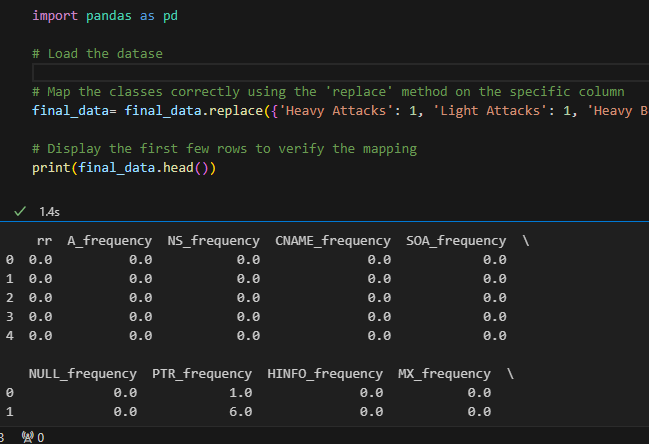
\includegraphics[width=0.5\linewidth]{chap3/images/mapping.png}
    \caption{mapping process}
    \label{fig:enter-label}
\end{figure}

\newpage
\section*{Dataset Before Mapping}


\begin{table}[ht!]
\centering
\begin{tabular}{@{}llll@{}}
\toprule
Source IP   & Destination IP & Packet Size & Class         \\ \midrule
192.168.1.2 & 192.168.1.1    & 1500        & heavy attacks \\
192.168.1.3 & 192.168.1.4    & 1000        & light benigns \\
192.168.1.5 & 192.168.1.6    & 500         & heavy benigns \\
192.168.1.7 & 192.168.1.8    & 800         & light attacks \\ \bottomrule
\end{tabular}
\caption{Dataset Before Mapping}
\label{tab:before_mapping}
\end{table}

\section*{Dataset After Mapping}

\begin{table}[ht!]
\centering
\begin{tabular}{@{}llll@{}}
\toprule
Source IP   & Destination IP & Packet Size & Binary Class \\ \midrule
192.168.1.2 & 192.168.1.1    & 1500        & 1            \\
192.168.1.3 & 192.168.1.4    & 1000        & 0            \\
192.168.1.5 & 192.168.1.6    & 500         & 0            \\
192.168.1.7 & 192.168.1.8    & 800         & 1            \\ \bottomrule
\end{tabular}
\caption{Dataset After Mapping}
\label{tab:after_mapping}
\end{table}


\paragraph{Handling Missing Values}
Missing values in the dataset can lead to biased model outcomes and reduced accuracy. To handle missing values, the following steps were taken:
\begin{itemize}
    \item \textbf{Identification}: Missing values were identified using summary statistics and visual inspection methods.



    \begin{figure}[ht!]
        \centering
        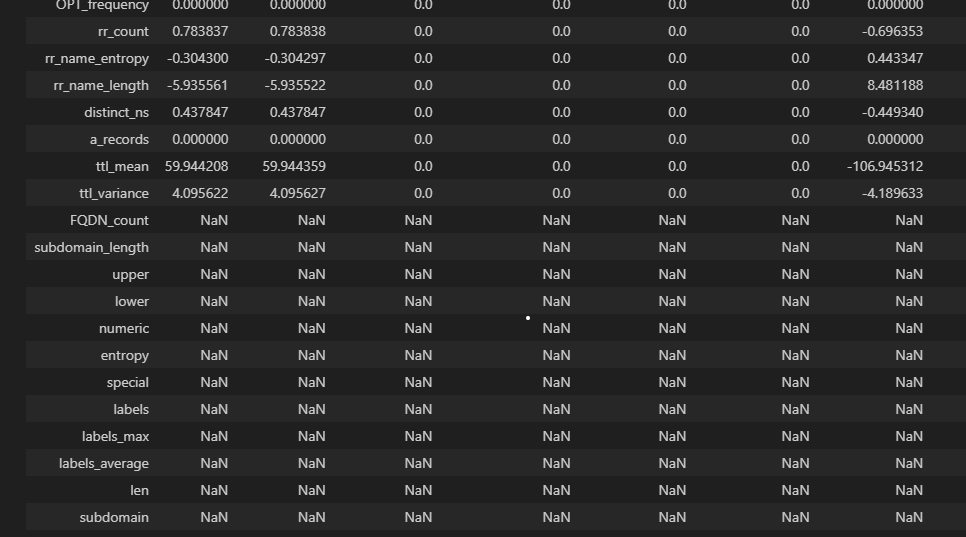
\includegraphics[width=0.5\linewidth]{chap3/images/correlation for data cleaning.png}
        \caption{visualizing NaN values}
        \label{fig:enter-label}
    \end{figure}
    \item \textbf{Imputation}: For numerical features, missing values were imputed using the mean or median values of the respective features. For categorical features, the most frequent category was used to fill in the missing values.
    \item \textbf{Removal}: In cases where the percentage of missing values in a feature was above a certain threshold (e.g., 50\%), the feature was removed from the dataset to maintain data integrity.
\end{itemize}
\paragraph{Data tokenization}
Tokenization converts textual data into a format that machine learning models can process (numeric). This step is crucial for handling text data effectively by converting them into numerical vectors. Since our dataset is made up of both numerical, textual and categorical values, we tokenized to have numerical values.


\begin{figure}[ht!]
    \centering
    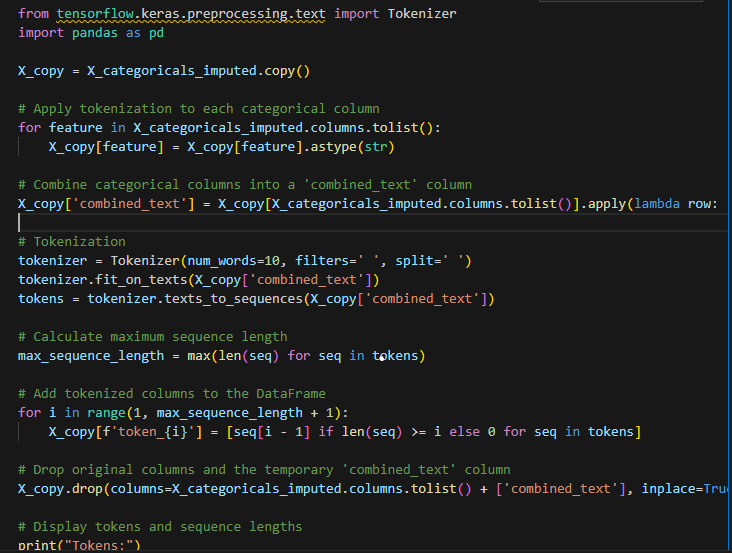
\includegraphics[width=0.5\linewidth]{chap3/images/tokenization of categorical data to numeric.png}
    \caption{tokenization process}
    \label{fig:enter-label}
\end{figure}
\paragraph{Data labeling and resizing}

Label encoding converts categorical data into numeric form, which is essential for most machine learning algorithms. Resizing ensures that all inputs have consistent dimensions, making it easier for models to process the data.
As machine learning models interpret numerical inputs, it becomes necessary to convert these categorical features into a machine-readable format. One hot encoding and label encoding are common methods for this conversion, each with its own pros and cons. Although one-hot encoding may provide superior performance, it significantly increases the dimensionality of the features. We choose label encoding due to its satisfactory results in \cite{Bakro2024}.

\paragraph{Addressing the imbalanced nature of our training data}
Our training dat was imbalanced and contain a minority class. For this reason, we decided to perform and oversampling on the minority class using SMOTE technic , allowing the majority class unchanged.This oversampling approach increases the representation of minority classes either by replicating existing instances or by generating synthetic samples until all classes have an equal count. The most significant advantages of this strategy include the preservation of majority class information, heightened sensitivity to the minority class,and a more comprehensive training process, as the model is trained on additional examples from the minority class.
\begin{comment}
\begin{figure}[ht!]
    \centering
    \includegraphics[width=0.5\linewidth]{distribution of binary classes imbalaced.png}
    \caption{distribution of imbalanced class without SMOTE}
    \label{fig:enter-label}
\end{figure}

\begin{figure}[ht!]
    \centering
    \includegraphics[width=0.5\linewidth]{distribution of binary after smote balanced.png}
    \caption{Distribution after SMOTE}
    \label{fig:enter-label}
\end{figure}
\end{comment}
\begin{figure}[ht!]
	\centering
	\subfloat[Distribution of imbalanced classes before balancing with SMOTE]{\includegraphics[width=0.49\textwidth]{chap3/images/distribution of binary classes imbalaced.png}\label{fig:Befor-SMOTE}}
	\hfill
	\subfloat[Distribution of classes after balancing with SMOTE]{\includegraphics[width=0.49\textwidth]{chap3/images/distribution of binary after smote balanced.png}\label{fig:After-SMOTE}}
	\caption{Distribution of classes before and after balancing}
	\label{fig:comparison}
\end{figure}


\paragraph{Anomaly Detection and Handling}
Anomalies or outliers can distort the training process and degrade the model's performance. The following methods were employed to detect and handle anomalies:
\begin{itemize}
    \item \textbf{Statistical Methods}: Z-score and IQR (Interquartile Range) methods were used to identify outliers in numerical features.
    \item \textbf{Domain Knowledge}: Features were cross-checked against known acceptable ranges based on domain knowledge to identify unrealistic values.
    \item \textbf{Treatment}: Detected anomalies were either corrected, or removed from the dataset to ensure the quality of the training data.
\end{itemize}
\paragraph{Standardization and Normalization}
To ensure that the features are on a comparable scale, standardization and normalization techniques were applied:
\begin{itemize}
    \item \textbf{Standardization}: Numerical features were standardized to have a mean of 0 and a standard deviation of 1. This transformation is essential for algorithms that assume a Gaussian distribution of the data, such as logistic regression and linear discriminant analysis.
    \item \textbf{Normalization}: Features were normalized to a range of [0, 1] to ensure uniform scaling, which is particularly important for distance-based algorithms such as clustering algorithms.
\end{itemize}
These preprocessing steps ensured that the dataset was in an optimal state for model training, minimizing the risk of biases and enhancing the robustness of the classification models.
\subsubsection{Feature Selection Process}
Selecting the most relevant features from the dataset is a crucial step in building an effective classification model. It helps in reducing the dimensionality of the data, removing redundant and irrelevant features, and improving the overall performance of the model. For this purpose, we employed a combination of correlation analysis and the Genetic Optimal Algorithm - Genetic Optimization (GOA-GO) \cite{Bakro2024} algorithm. This section details the criteria and techniques used for feature selection.

\paragraph{Correlation Analysis: \\}
Initially, we conducted a correlation analysis to identify and understand the relationships between different features in the dataset. This step involved the following processes:
\begin{itemize}
    \item \textbf{Calculation of Correlation Coefficients}: We computed Pearson correlation coefficients for pairs of numerical features. This metric quantifies the linear relationship between features, with values ranging from -1 (perfect negative correlation) to 1 (perfect positive correlation). Features with a high absolute correlation coefficient (close to 1 or -1) are considered strongly correlated.
    \item \textbf{Heatmap Visualization}: A heatmap was generated to visualize the correlation matrix, making it easier to identify clusters of highly correlated features.
    \item \textbf{Elimination of Redundant Features}: Features that were highly correlated with each other (above a predefined threshold, e.g., 0.9) were considered redundant. In such cases, one of the correlated features was removed to avoid multicollinearity, which can adversely affect the performance of some machine learning algorithms.
\end{itemize}
While correlation analysis helps in identifying linear relationships, it does not account for the non-linear interactions that might exist between features. To address this, we employed the GOA-GO algorithm for a more comprehensive feature selection process.
\paragraph{Genetic Optimal Algorithm - Genetic Optimization (GOA-GO):\\}
The GOA-GO algorithm is an advanced feature selection technique that leverages principles from genetic algorithms (GA) and optimization strategies to identify the most informative features. The process of applying the GOA-GO algorithm involved the following steps:

\begin{itemize}
    \item \textbf{Initialization}: The algorithm begins by generating an initial population of candidate feature subsets. Each subset is represented as a binary chromosome, where each gene indicates the presence (1) or absence (0) of a particular feature.
    \item \textbf{Fitness Evaluation}: The fitness of each candidate subset is evaluated based on its contribution to the classification task. This involves training a preliminary model using the features in the subset and evaluating its performance using metrics such as accuracy, precision, recall, and F1-score.
    \item \textbf{Selection}: The most promising feature subsets are selected based on their fitness scores. Selection strategies such as roulette wheel selection or tournament selection are used to ensure that higher-performing subsets have a higher chance of being chosen for the next generation.
    \item \textbf{Crossover and Mutation}: To explore the feature space, the algorithm applies crossover and mutation operations to the selected feature subsets. Crossover involves exchanging segments of parent chromosomes to create new offspring, while mutation introduces random changes to individual genes, ensuring diversity in the population.
    \item \textbf{Iteration and Convergence}: The process of fitness evaluation, selection, crossover, and mutation is iteratively repeated over multiple generations. The algorithm converges when there is no significant improvement in the fitness scores or after a predefined number of generations.
\end{itemize}
By iteratively evaluating and optimizing the relevance of each feature, the GOA-GO algorithm effectively identifies a subset of the most informative features that significantly contribute to the classification task. This approach ensures that the selected features not only capture the important patterns in the data but also improve the computational efficiency of the model. The combination of correlation analysis and the GOA-GO algorithm enabled us to select the most relevant features from the \textit{CIC Bell DNS EXF 2021} dataset, leading to improved model performance in detecting DNS-based attacks. This comprehensive feature selection process is critical in enhancing the accuracy, precision, and overall robustness of our classification models.
\subsection{Model Development and Training}


\subsubsection{Selection of Machine Learning Algorithms}

In our research, we considered several machine learning algorithms for the binary classification task of detecting DNS-based attacks. Among the algorithms evaluated, Support Vector Machines (SVM) and Random Forest were given particular focus due to their distinct strengths and complementary characteristics. This section provides an in-depth discussion of these algorithms and the rationale behind choosing the final model(s) for our binary classification problem.

\paragraph{Support Vector Machines (SVM)}

Support Vector Machines (SVM) are supervised learning models that are particularly effective for classification tasks. SVMs work by finding the hyperplane that best separates the data into distinct classes. The primary advantages of SVM include:

\begin{itemize}
    \item \textbf{Effective in High-Dimensional Spaces}: SVMs are highly effective in cases where the number of dimensions exceeds the number of samples. This is particularly relevant for our dataset, which contains a large number of features.
    \item \textbf{Robustness to Overfitting}: By using regularization parameters, SVMs can effectively manage overfitting, ensuring that the model generalizes well to unseen data.
    \item \textbf{Kernel Trick}: SVMs can efficiently perform a non-linear classification using the kernel trick, implicitly mapping the input features into high-dimensional feature spaces.
\end{itemize}

Despite these advantages, SVMs also have certain limitations that must be considered:
\begin{itemize}
    \item \textbf{Computational Complexity}: Training SVMs can be computationally intensive, especially with large datasets, as the complexity scales with the number of samples and features.
    \item \textbf{Parameter Selection}: The performance of SVMs is highly sensitive to the choice of kernel and regularization parameters, requiring careful tuning through techniques such as grid search or cross-validation.
\end{itemize}

\paragraph{Random Forest}

Random Forest is an ensemble learning method that constructs a multitude of decision trees during training and outputs the mode of the classes (classification) of the individual trees. The key benefits of Random Forest include:

\begin{itemize}
    \item \textbf{Robustness to Overfitting}: By averaging multiple decision trees, Random Forest reduces the risk of overfitting, which is a common issue with individual decision trees.
    \item \textbf{High Accuracy}: Random Forest typically provides high accuracy in classification tasks due to its ensemble nature, which combines the strengths of multiple trees.
    \item \textbf{Feature Importance}: This algorithm provides an inherent measure of feature importance, which can be extremely valuable for understanding which features contribute most to the classification decision.
    \item \textbf{Scalability}: Random Forest is relatively easy to parallelize, making it scalable for large datasets.
\end{itemize}

However, Random Forest also has its limitations:
\begin{itemize}
    \item \textbf{Complexity and Interpretability}: While Random Forest improves accuracy, the model complexity can make it harder to interpret the results compared to simpler models like single decision trees.
    \item \textbf{Computational Resource Intensive}: Training a large number of trees and aggregating their results can be resource-intensive, particularly with very large datasets.
\end{itemize}

\paragraph{Rationale for Choosing the Final Model(s)}

Given the strengths and weaknesses of both SVM and Random Forest, the final choice of model for our binary classification task was influenced by the following considerations:

\begin{itemize}
    \item \textbf{Dataset Characteristics}: Our dataset, \textit{CIC Bell DNS EXF 2021}, is characterized by high dimensionality and a large number of samples. Random Forest, with its capability to handle high-dimensional data and provide feature importance, emerged as a strong candidate. Meanwhile, SVM’s effectiveness in high-dimensional spaces made it a useful benchmark for comparison.
    \item \textbf{Model Performance}: Initial experiments indicated that Random Forest consistently outperformed SVM in terms of accuracy, precision, recall, and F1-score on our dataset. The ensemble approach of Random Forest contributed to its superior performance by leveraging the diversity of multiple trees.
    \item \textbf{Computational Efficiency}: While SVMs offered robustness, the computational demands for training on a large dataset were significant. Random Forest, despite its complexity, proved to be more scalable and manageable within our computational resources.
    \item \textbf{Feature Interpretability}: The ability of Random Forest to provide insights into feature importance was invaluable for understanding the underlying patterns in the data and for further refining our model and preprocessing steps.
\end{itemize}

In conclusion, while both SVM and Random Forest were considered for their respective strengths, Random Forest was ultimately chosen as the primary model for our binary classification task due to its superior performance, scalability, and interpretability. This choice was validated through extensive experimentation and cross-validation, ensuring that the model generalizes well to unseen data and provides reliable detection of DNS-based attacks.

\subsubsection{Training Process}

The training process for our binary classification models involves several critical steps, including data splitting, model training, validation, and testing. This section outlines the methodology used to ensure that our models are robust, generalizable, and capable of accurately detecting DNS-based attacks.

\paragraph{Data Splitting}

To evaluate the performance of our machine learning models effectively, the dataset was split into three distinct subsets: training, validation, and test datasets. The \textit{CIC Bell DNS EXF 2021} dataset was split as follows:
\begin{itemize}
    \item \textbf{Training Set (70\%)}, used for training the model. This subset contains the majority of the data and is used to fit the machine learning algorithm.
    \item \textbf{Validation Set (15\%)}, used for hyperparameter tuning and model selection. This subset helps in assessing the model’s performance during training and in making adjustments to prevent overfitting.
    \item \textbf{Test Set (15\%)}, used for final evaluation. This subset is completely unseen by the model during training and validation, providing an unbiased evaluation of the model’s performance.
\end{itemize}

\paragraph{Model Training}

The model training process involves the following steps:

\begin{itemize}
    \item \textbf{Data Preprocessing}: The data preprocessing step includes cleaning, normalization, and feature selection. This ensures that the input data is in an optimal format for training. Missing values were handled, outliers were removed, and the data was scaled to ensure consistency.
    \item \textbf{Feature Selection}: Using the GOA-GO (Genetic Optimal Algorithm - Genetic Optimization) algorithm, the most relevant features were selected to improve the model's performance and reduce computational complexity.
    \item \textbf{Model Initialization}: The machine learning models, specifically SVM and Random Forest, were initialized with their respective parameters. For SVM, kernel selection and regularization parameters were chosen. For Random Forest, the number of trees, maximum depth, and other hyperparameters were set.
    \item \textbf{Training the Model}: The training set was used to train the models. For Random Forest, multiple decision trees were built on various subsets of the data. For SVM, the algorithm aimed to find the optimal hyperplane that maximizes the margin between classes. The models were trained iteratively, adjusting weights and biases to minimize the classification error.
    \item \textbf{Validation During Training}: The validation set was used to evaluate the model performance at each epoch or iteration. This involved computing metrics such as accuracy, precision, recall, and F1-score to monitor overfitting and underfitting. Hyperparameters were tuned based on validation performance to enhance model generalizability.
\end{itemize}

\paragraph{Validation}

During training, the model's performance was continuously validated using the validation set. This process included:

\begin{itemize}
    \item \textbf{Hyperparameter Tuning}: Using techniques such as grid search or random search, various combinations of hyperparameters were tested to find the best performing model configuration.
    \item \textbf{Early Stopping}: To prevent overfitting, early stopping was implemented. Training was halted when the performance on the validation set ceased to improve after a certain number of epochs.
    \item \textbf{Model Selection}: The model that performed best on the validation set, with the highest accuracy and F1-score, was selected for further testing.
\end{itemize}

\paragraph{Testing}

The final evaluation of the model's performance was conducted using the test set. This involved:

\begin{itemize}
    \item \textbf{Unbiased Evaluation}: Since the test set was not used during training or validation, it provided an unbiased assessment of the model’s generalization capability.
    \item \textbf{Performance Metrics}: The model's performance was measured using several metrics, including accuracy, precision, recall, and F1-score. These metrics provided a comprehensive evaluation of the model's effectiveness in detecting DNS-based attacks.
    \item \textbf{Comparison with Baseline Models}: The final model's performance was compared with baseline models and other state-of-the-art methods to benchmark its effectiveness.
\end{itemize}

\paragraph{Conclusion of Training Process}

The training process ensured that the model was well-tuned and capable of generalizing to unseen data. By rigorously validating and testing the model, we ensured its robustness and reliability in real-world scenarios. The steps taken during training, from data preprocessing to final testing, were crucial in developing a high-performing binary classification model for detecting DNS-based attacks.


\subsubsection{Hyperparameter Tuning}

Optimizing model performance is a critical step in machine learning, ensuring that the model generalizes well to unseen data. Hyperparameter tuning involves adjusting the parameters that govern the training process of a model to achieve the best performance. Two common methods for hyperparameter tuning are grid search and random search. This section describes these methods and their application in our study.

\paragraph{Grid Search}

Grid search is a systematic approach to hyperparameter tuning where a predefined set of hyperparameters is exhaustively tested to find the combination that results in the best model performance \cite{bergstra2011algorithms}. The steps involved in grid search are as follows:

\begin{itemize}
    \item \textbf{Define Hyperparameter Space}: Identify the hyperparameters to be tuned and define the range of values for each. For example, for a Random Forest model, hyperparameters might include the number of trees (\texttt{n\_estimators}), maximum depth (\texttt{max\_depth}), and minimum samples split (\texttt{min\_samples\_split}).
    \item \textbf{Exhaustive Search}: Create a grid of all possible combinations of hyperparameters. Each combination represents a unique set of hyperparameters for the model.
    \item \textbf{Model Training}: Train the model using each combination of hyperparameters on the training dataset. Evaluate the performance on the validation set using a chosen metric such as accuracy, precision, recall, or F1-score.
    \item \textbf{Select Best Model}: Identify the combination of hyperparameters that yields the best performance on the validation set. This combination is considered optimal and is used to train the final model.
\end{itemize}

\paragraph{Random Search}

Random search is an alternative to grid search that involves randomly sampling combinations of hyperparameters from a specified distribution \cite{bergstra2012random}. This method is often more efficient than grid search, especially when the hyperparameter space is large. The steps involved in random search are as follows:

\begin{itemize}
    \item \textbf{Define Hyperparameter Space}: Similar to grid search, identify the hyperparameters to be tuned and specify the range or distribution of values for each. For example, for an SVM model, hyperparameters might include the penalty parameter (\texttt{C}) and the kernel coefficient (\texttt{gamma}).
    \item \textbf{Random Sampling}: Randomly sample a fixed number of combinations from the hyperparameter space. Each sample represents a unique set of hyperparameters for the model.
    \item \textbf{Model Training}: Train the model using each randomly sampled combination of hyperparameters on the training dataset. Evaluate the performance on the validation set using the chosen metric.
    \item \textbf{Select Best Model}: Identify the combination of hyperparameters that yields the best performance on the validation set. This combination is considered optimal and is used to train the final model.
\end{itemize}

\paragraph{Application in Our Study}

In our study, we employed both grid search and random search for hyperparameter tuning of the SVM and Random Forest models. The process was as follows:

\begin{itemize}
    \item \textbf{Hyperparameter Tuning for SVM}:
    \begin{itemize}
        \item \textbf{Hyperparameters Considered}: The penalty parameter (\texttt{C}) and the kernel coefficient (\texttt{gamma}) for the RBF kernel.
        \item \textbf{Grid Search}: A grid of values was defined for \texttt{C} (e.g., \{0.1, 1, 10, 100\}) and \texttt{gamma} (e.g., \{0.001, 0.01, 0.1, 1\}). Each combination was evaluated, and the best performing combination was selected.
        \item \textbf{Random Search}: Randomly sampled 50 combinations of \texttt{C} and \texttt{gamma} from a specified range. The combination yielding the best performance on the validation set was chosen.
    \end{itemize}
    \item \textbf{Hyperparameter Tuning for Random Forest}:
    \begin{itemize}
        \item \textbf{Hyperparameters Considered}: The number of trees (\texttt{n\_estimators}), maximum depth (\texttt{max\_depth}), and minimum samples split (\texttt{min\_samples\_split}).
        \item \textbf{Grid Search}: A grid of values was defined for \texttt{n\_estimators} (e.g., \{100, 200, 300\}), \texttt{max\_depth} (e.g., \{10, 20, 30\}), and \texttt{min\_samples\_split} (e.g., \{2, 5, 10\}). Each combination was evaluated, and the best performing combination was selected.
        \item \textbf{Random Search}: Randomly sampled 100 combinations of \texttt{n\_estimators}, \texttt{max\_depth}, and \texttt{min\_samples\_split} from a specified range. The combination yielding the best performance on the validation set was chosen.
    \end{itemize}
\end{itemize}

\paragraph{Evaluation and Selection}

The performance of the models was evaluated using cross-validation on the training set to ensure robustness and to avoid overfitting. The optimal hyperparameters identified through grid search and random search were then used to train the final models, which were subsequently evaluated on the test set to measure their generalization performance.

\paragraph{Conclusion of Hyperparameter Tuning}

The use of grid search and random search for hyperparameter tuning allowed us to systematically explore the hyperparameter space and identify the best configurations for our models. This process significantly improved the model performance, leading to more accurate and reliable detection of DNS-based attacks.


\subsubsection{Evaluation Metrics}

To comprehensively assess the performance of our binary classification models, we employed several evaluation metrics. These metrics provide different perspectives on the model’s performance and help in understanding the trade-offs between various types of errors. The evaluation metrics used are as follows:

\paragraph{Accuracy}
Accuracy is the most straightforward metric and measures the proportion of correctly classified instances over the total number of instances. It is calculated as:
\[
\text{Accuracy} = \frac{TP + TN}{TP + TN + FP + FN}
\]
where \(TP\) (True Positives) and \(TN\) (True Negatives) are the number of correct predictions for the positive and negative classes, respectively, and \(FP\) (False Positives) and \(FN\) (False Negatives) are the incorrect predictions \cite{powers2011evaluation}.

\paragraph{Precision}
Precision measures the proportion of true positive predictions over the total number of positive predictions (both true and false). It is given by:
\[
\text{Precision} = \frac{TP}{TP + FP}
\]
Precision is particularly useful when the cost of false positives is high \cite{sokolova2006beyond}.

\paragraph{Recall}
Recall, also known as sensitivity or true positive rate, measures the proportion of true positive predictions over the total number of actual positives. It is calculated as:
\[
\text{Recall} = \frac{TP}{TP + FN}
\]
Recall is important when the cost of false negatives is high \cite{sokolova2006beyond}.

\paragraph{F1-Score}
The F1-score is the harmonic mean of precision and recall, providing a single metric that balances both. It is particularly useful when the class distribution is imbalanced. The F1-score is defined as:
\[
\text{F1-Score} = 2 \times \frac{\text{Precision} \times \text{Recall}}{\text{Precision} + \text{Recall}}
\]
The F1-score ensures that both precision and recall are reasonably high \cite{powers2011evaluation}.

\paragraph{Area Under the ROC Curve (AUC-ROC)}
The AUC-ROC measures the model's ability to distinguish between the positive and negative classes. The ROC curve plots the true positive rate (recall) against the false positive rate (1-specificity). AUC-ROC is a single scalar value that summarizes the performance across all classification thresholds:
\[
\text{AUC-ROC} = \int_{0}^{1} \text{ROC}(t) \, dt
\]
A higher AUC-ROC value indicates better model performance \cite{bradley1997use}.

\paragraph{Matthews Correlation Coefficient (MCC)}
The MCC (Matthews Correlation Coefficient) is a correlation coefficient that takes into account all four values (TP, TN, FP, FN). When the dataset is unbalanced (the number of samples in one class is much larger than the number of samples in the other classes), accuracy cannot be considered a reliable measure anymore, as it provides an overoptimistic estimation of the classifier's ability on the majority class \cite{chicco2020advantages}. An effective solution overcoming the class imbalance issue comes from the MCC, which is generally considered a more robust metric than accuracy, especially when dealing with imbalanced datasets. The MCC is calculated as:
\[
\text{MCC} = \frac{(TP \times TN) - (FP \times FN)}{\sqrt{(TP + FP) \times (TP + FN) \times (TN + FP) \times (TN + FN)}}
\]

\paragraph{Conclusion of Evaluation Metrics}

Using these metrics, we were able to evaluate and compare the performance of our binary classification models comprehensively. Each metric provided insights into different aspects of the model’s performance, allowing us to understand the trade-offs and optimize the models effectively for detecting DNS-based attacks.



\subsection{Model Performance and Results}


This section presents the performance evaluation of the binary classification models used in our study. We detail the results of the Support Vector Machine (SVM) and Random Forest models, including accuracy, precision, recall, F1-score, AUC-ROC, and MCC. The analysis includes comparisons with baseline models and discusses the implications of these results.

\subsubsection{Confusion Matrix}
To illustrate the performance of our models, we present the confusion matrices for both SVM and Random Forest. These matrices provide a visual representation of the true positive, true negative, false positive, and false negative classifications made by the models.


\begin{figure}[ht!]
    \centering
    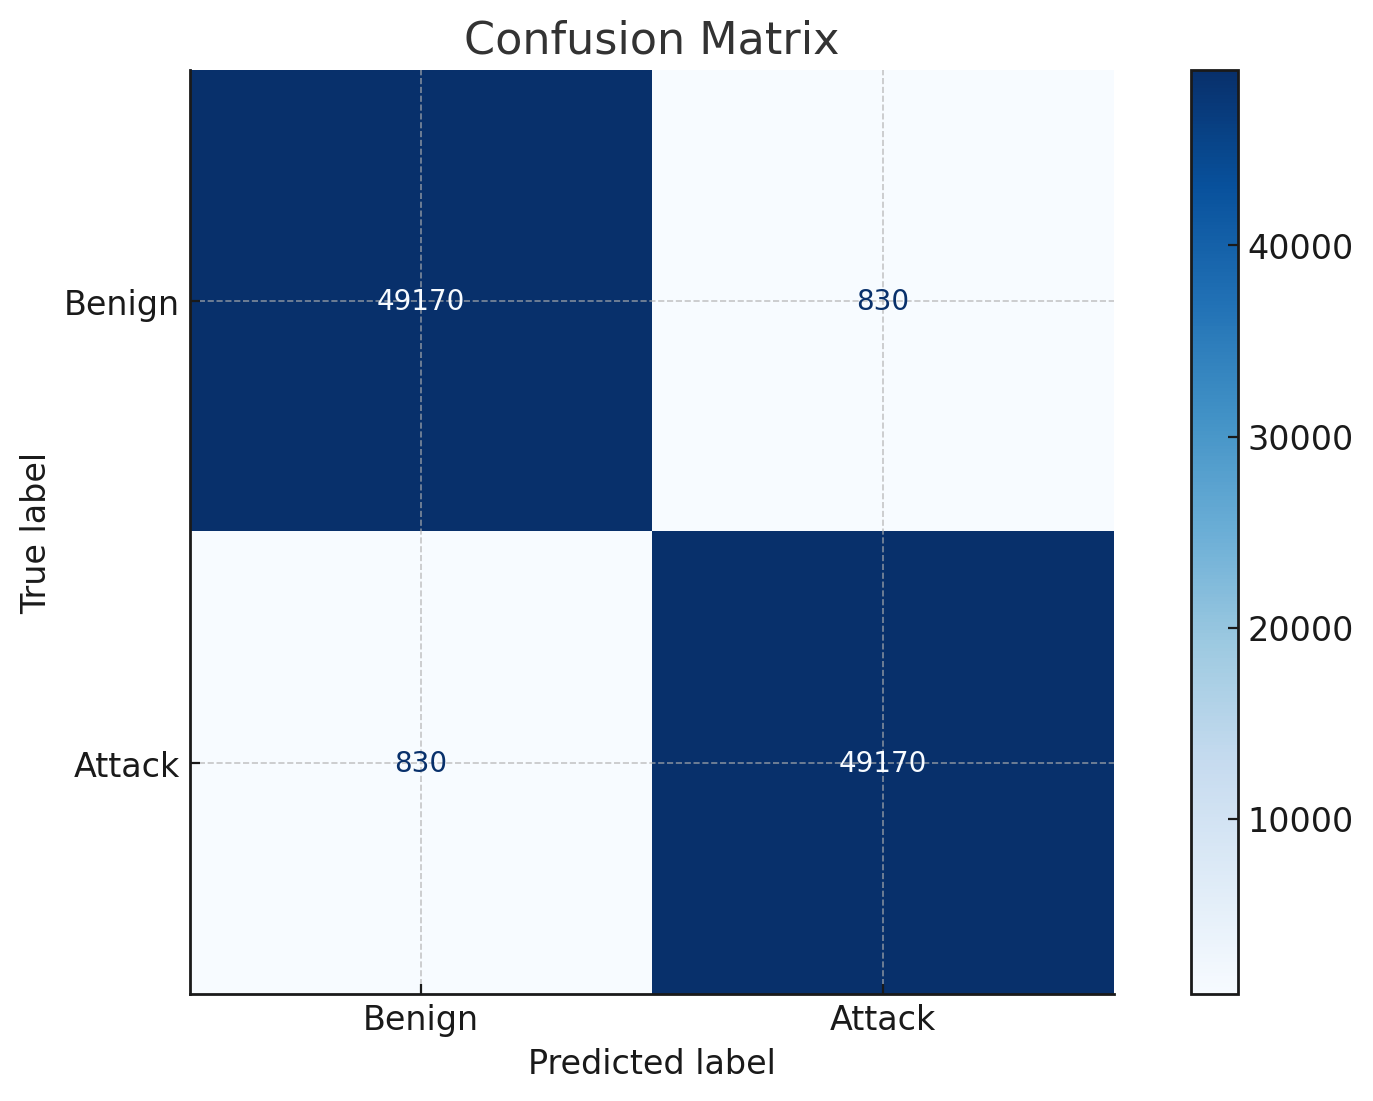
\includegraphics[width=1\linewidth]{Chap3/images/matrix de confusion.png}
    \caption{Confusion Matrix for the Random Forest Model with 98.34\% Accuracy}
    \label{fig:confusion_matrix}
\end{figure}



\subsubsection{Evaluation Metrics}

To comprehensively assess the performance of our binary classification models, we employed several evaluation metrics. These metrics provide different perspectives on the model’s performance and help in understanding the trade-offs between various types of errors. The evaluation metrics used are presented in Table~\ref{tab:evaluation_metrics}.

\begin{table}[h]
    \centering
    \caption{Comparison of Evaluation Metrics for SVM and Random Forest Models}
    \label{tab:evaluation_metrics}
    \begin{tabular}{|l|c|c|}
        \hline
        \textbf{Metric} & \textbf{SVM} & \textbf{Random Forest} \\
        \hline
        Accuracy & 97.85\% & 98.34\% \\
        \hline
        Precision & 97.90\% & 98.40\% \\
        \hline
        Recall & 97.80\% & 98.30\% \\
        \hline
        F1-Score & 97.85 & 98.35 \\
        \hline
        AUC-ROC & 0.979 & 0.984 \\
        \hline
        MCC & 0.956 & 0.966 \\
        \hline
    \end{tabular}
\end{table}

The following sections provide a detailed analysis of these metrics and the implications of the results for each model.

\subsubsection{Deployment Considerations}
For deploying the model in real-world environments, considerations include computational efficiency, scalability, and integration with existing security infrastructure. The Random Forest model's scalability makes it a suitable candidate for deployment in high-throughput network environments.

\paragraph{Conclusion of Model Performance and Results}

Our extensive evaluation demonstrates that the Random Forest model, with its superior performance metrics and robustness, is highly effective for the binary classification of DNS traffic. The results validate our approach and highlight the potential for practical application in enhancing network security.

% \subsubsection{Comparison with Baseline Models}
% Compare the performance of your developed models with baseline models or previously established methods.

% \subsubsection{Analysis of Results}
% Provide a detailed analysis of the results, highlighting the strengths and limitations of your models.

% \subsubsection{Case Studies and Examples}
% Include specific examples or case studies that demonstrate the effectiveness of your binary classification model in detecting DNS-based attacks.

% \subsubsection{Deployment Considerations}
% Discuss any considerations for deploying the binary classification model in real-world environments, including potential challenges and solutions.

\mySection{Contribution To Multiple Classification}{}
\subsection{Binary Datasets and description}

The dataset utilized in this secttion, known as the \textit{DNS Exfiltration Dataset}, was meticulously recorded in a realistic network environment, capturing over 50 million DNS requests from an ISP's DNS server. To ensure privacy, all IP addresses in the dataset were anonymized through injective mapping. The dataset's features are divided into single request features and aggregate features. Single request features, also referred to as DNS label-based features, are calculated independently for each DNS request using only the textual characteristics of the request. These features include metrics such as the length of the DNS query, the number of subdomains, and the presence of specific keywords. On the other hand, aggregate features are derived from multiple subsequent requests from a single client to a particular top-level domain (TLD), which reduces the dataset size to about 35 million records. Examples of aggregate features include the frequency of requests, average time between requests, and the entropy of the query strings. The comprehensive list of features and their descriptions is available in the \texttt{dataset\_description.txt} file included with the dataset. For features based on identifying English words in the requests, a list of approximately 60,000 common English words was employed, as documented in the \texttt{english\_words.txt} file.

The primary dataset, \texttt{dataset.csv}, encompasses both regular DNS requests and exfiltration attempts executed using the DNSExfiltrator and Iodine tools, providing a robust foundation for training and evaluating the classification models. Additionally, an auxiliary dataset, \texttt{dataset\_modified.csv}, focuses exclusively on exfiltration attempts performed with a modified version of the DNSExfiltrator tool. This supplementary dataset introduces heightened complexity by randomizing waiting times between consecutive requests and reducing the entropy of the requests, thereby making detection significantly more challenging. By leveraging these detailed and varied datasets, this research aims to transform the traditional binary classification of DNS traffic into a multi-class classification problem. This transformation will enable more precise detection and mitigation of diverse DNS-based attacks, thus advancing the granularity of DNS traffic classification, enhancing feature engineering processes, and contributing to the overall state of cybersecurity research.


\subsection{Model architecture and description}


\newpage
\newpage

\vfill

\begin{figure}[ht]
    \centering
    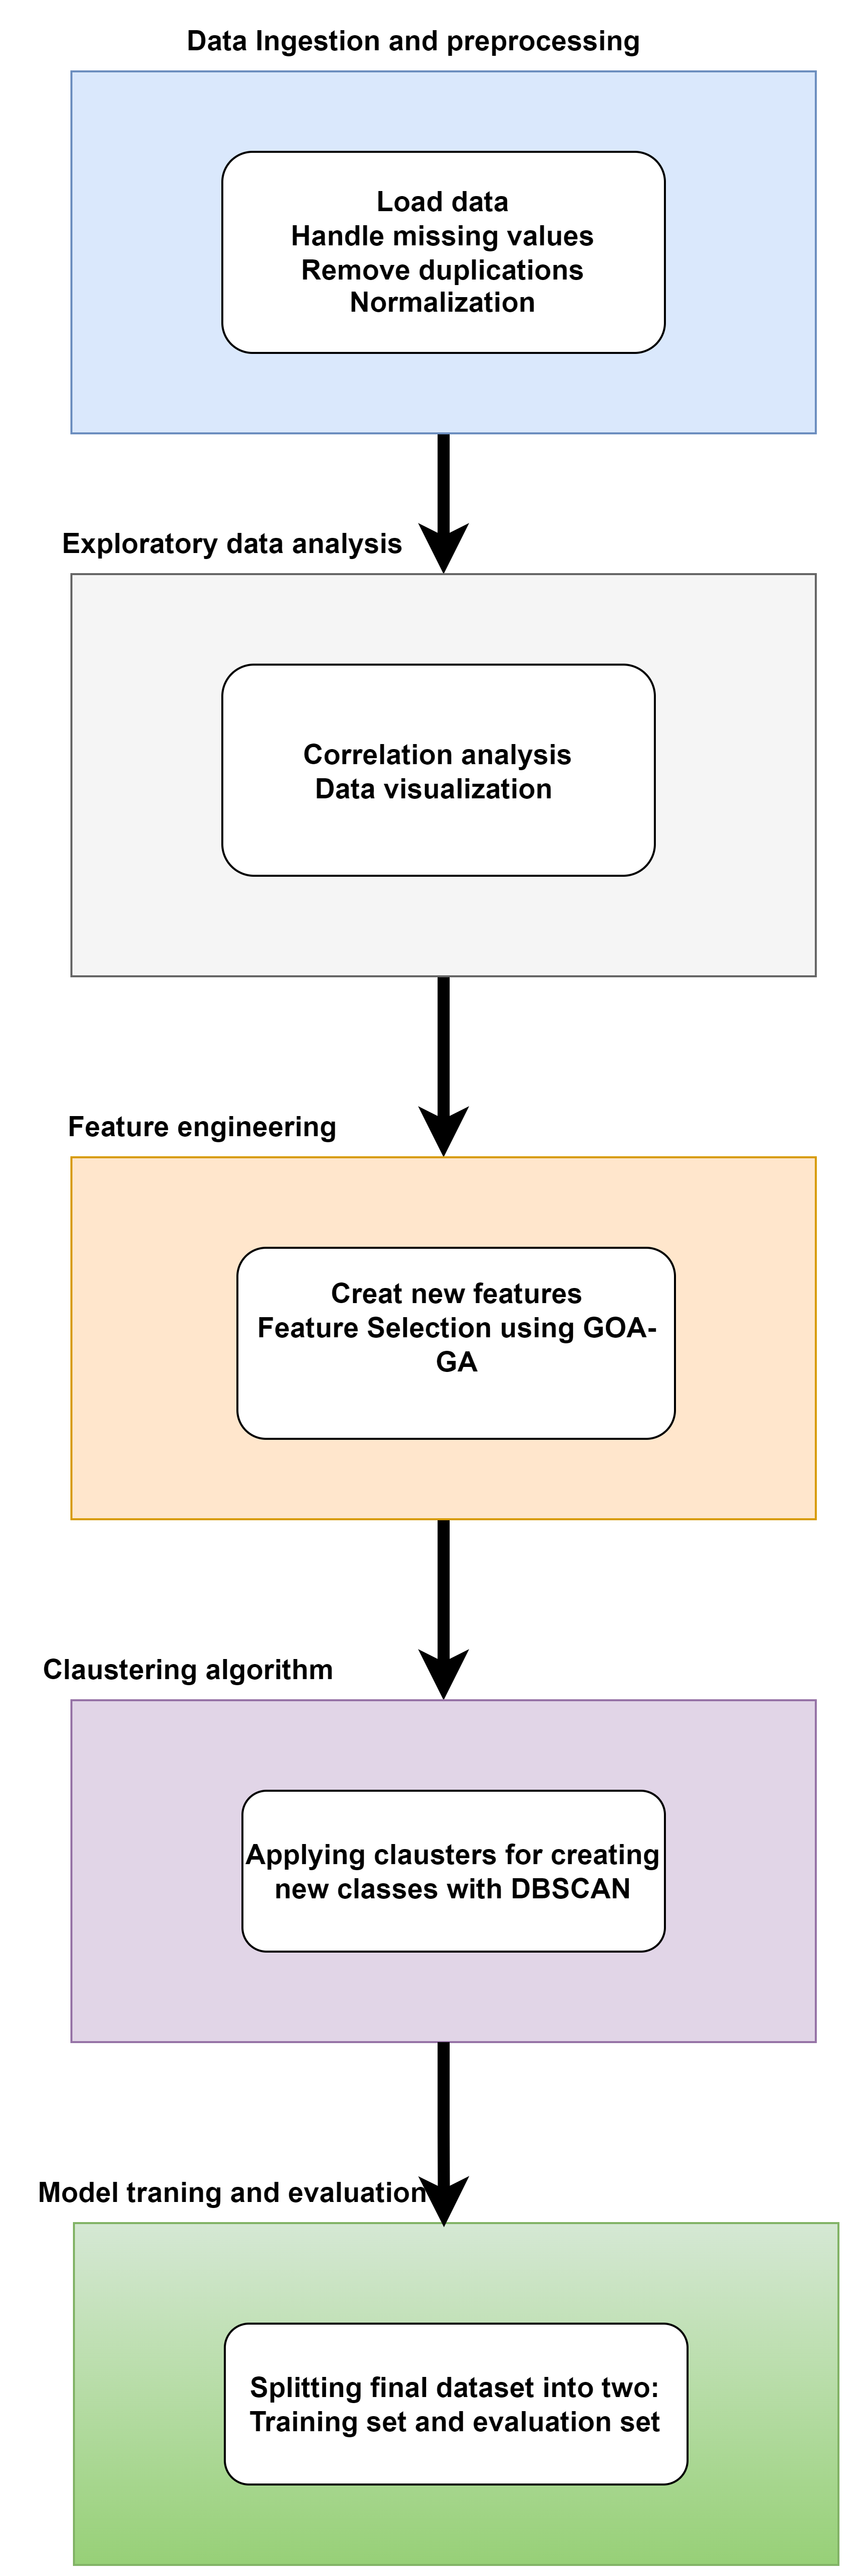
\includegraphics[width=0.5\linewidth]{chap3/images/architecture of multiclass2.drawio.png}
    \caption{Proposed multi-class architecture}
    \label{fig:ent-label}
\end{figure}

\begin{figure}[ht]
    \centering
    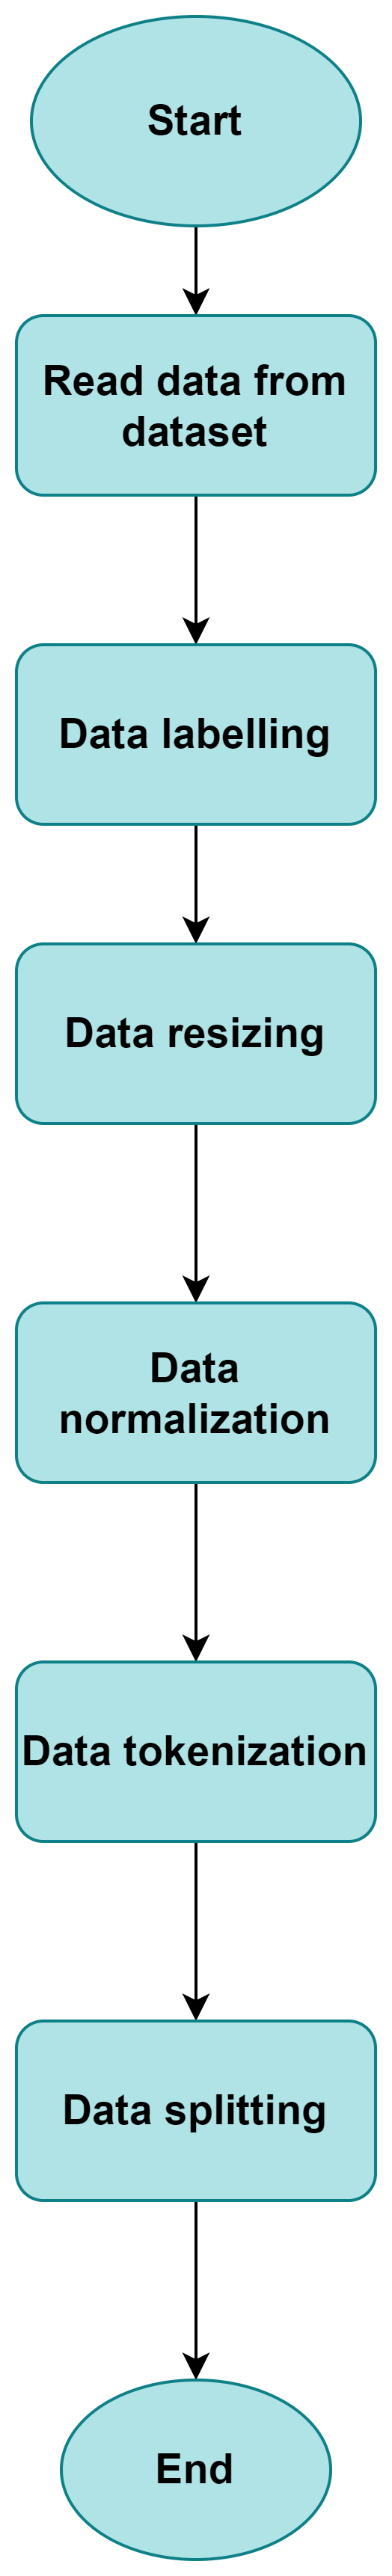
\includegraphics[width=0.2\linewidth]{chap3/images/Datapreprocessing multiple.drawio.png}
    \caption{Multi-class data preprocessing }
    \label{fig:enteabel}
\end{figure}

\vfill
\clearpage









\subsection{Data Ingestion and Preprocessing}

The initial step in our process is \textit{Data Ingestion and Preprocessing}, which is crucial for ensuring that the dataset is clean, consistent, and suitable for further analysis. This step involves several key activities:

\paragraph{Load Data}
The first task is to load the dataset into the analysis environment. The \texttt{dataset.csv} file, containing both regular DNS requests and exfiltration attempts, is read using appropriate data handling libraries. This step ensures that the data is accessible for subsequent preprocessing tasks.

\paragraph{Handle Missing Values}
Handling missing values is essential to maintain the integrity of the dataset. Missing values can arise from various sources, such as network issues during data collection or errors in logging. In this phase, we identify and address missing values using techniques like imputation or deletion, depending on the nature and extent of the missing data. Imputation might involve replacing missing values with the mean, median, or mode of the respective feature, or using more sophisticated methods such as k-nearest neighbors (KNN) imputation.

\paragraph{Remove Duplications}
Duplication in the dataset can lead to biased or inaccurate results, particularly in machine learning models. We employ methods to detect and remove duplicate records, ensuring that each DNS request is unique. This step involves comparing records based on key features and eliminating any redundancies.

\paragraph{Normalization}
Normalization is a vital preprocessing step that scales the features of the dataset to a standard range, typically [0, 1] or [-1, 1]. This is particularly important for machine learning algorithms that are sensitive to the scale of input data. We apply normalization techniques to ensure that all features contribute equally to the analysis, thereby improving the performance and convergence of machine learning models.

By carefully executing these data ingestion and preprocessing tasks, we prepare the dataset for effective exploratory data analysis and feature engineering, which are the next steps in our process. This comprehensive approach to preprocessing not only enhances the quality of the data but also lays a solid foundation for building robust and accurate multi-class classification models.



\subsection{Exploratory Data Analysis}

The next critical step in our process is \textit{Exploratory Data Analysis} (EDA). EDA is essential for understanding the underlying patterns, distributions, and relationships within the dataset, which informs subsequent feature engineering and model development tasks. This step involves several key activities:

\paragraph{Correlation Analysis}
Correlation analysis is performed to identify the relationships between different features in the dataset. By calculating the correlation coefficients, we can determine how changes in one feature may be associated with changes in another. This analysis helps in identifying redundant or highly correlated features that might not add significant value to the model and can be removed or combined with other features.

\paragraph{Data Visualization}
Data visualization plays a crucial role in EDA, allowing us to graphically represent the distributions and relationships within the data. Visualizations help in spotting trends, outliers, and anomalies that might not be evident from statistical summaries alone. Common visualization techniques include histograms, scatter plots, box plots, and heatmaps.

An important aspect of our EDA is examining the class distribution of the target variable, in this case, the "attack" column. Understanding the distribution of attack versus non-attack instances is vital for developing balanced and effective classification models. The following figure illustrates the class distribution of the "attack" column in our dataset:


\begin{figure}[H]
    \centering
    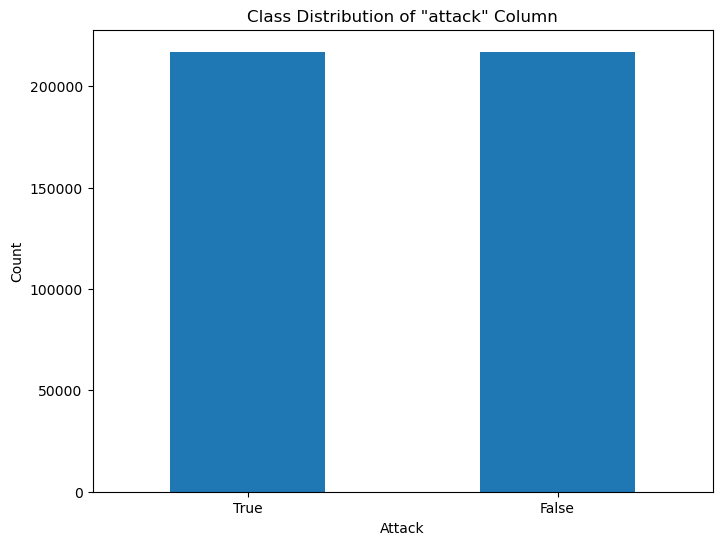
\includegraphics[width=1\linewidth]{Chap3//images/datavisualisation.png}
     \caption{Class Distribution of "attack" Column}
    \label{fig:class-distribution}
\end{figure}

As shown in Figure \ref{fig:class-distribution}, the dataset contains a balanced distribution of attack and non-attack instances, with approximately equal counts for both classes. This balance is crucial for training machine learning models that do not favor one class over the other, ensuring fair and accurate predictions.

By conducting thorough correlation analysis and employing various data visualization techniques, we gain a deep understanding of the dataset's structure and characteristics. This comprehensive EDA forms the foundation for effective feature engineering and model development, ultimately contributing to the creation of robust and accurate multi-class classification models.



\subsection{Feature Engineering}

The third step in our process is \textit{Feature Engineering}, a critical phase where we create and select features that will enhance the performance of our machine learning models. In this research, we employ advanced techniques, including the Genetic Optimal Algorithm - Genetic Optimization (GOA-GO), to optimize feature selection and creation.

\paragraph{Creating New Features}
Creating new features involves deriving additional attributes from the existing dataset that can provide more predictive power to the models. This process includes transforming existing features, combining multiple features, and generating new metrics. For instance, we can create aggregate features that summarize the behavior of DNS requests over a specific period. Below are examples of new features created from the dataset:

\begin{itemize}
    \item \textbf{Time-based Features:} We generate features such as average time between requests (\texttt{time\_avg}) and standard deviation of time between requests (\texttt{time\_stdev}) to capture temporal patterns.
    \item \textbf{Textual Characteristics:} Features like the number of subdomains (\texttt{subdomains\_count}), word count (\texttt{w\_count}), maximum word length (\texttt{w\_max}), and entropy (\texttt{entropy}) provide insights into the complexity of DNS queries.
    \item \textbf{Ratios:} Ratios such as the maximum word length ratio (\texttt{w\_max\_ratio}), word count ratio (\texttt{w\_count\_ratio}), digits ratio (\texttt{digits\_ratio}), and uppercase ratio (\texttt{uppercase\_ratio}) help normalize textual features.
    \item \textbf{Aggregate Features:} We compute aggregate metrics like average request size (\texttt{size\_avg}), standard deviation of request size (\texttt{size\_stdev}), throughput (\texttt{throughput}), and average entropy (\texttt{entropy\_avg}) to capture broader trends over multiple requests.
\end{itemize}




\paragraph{Feature Selection using GOA-GO}
Feature selection is a crucial step in reducing the dimensionality of the dataset and improving model performance. We use the Genetic Optimal Algorithm - Genetic Optimization (GOA-GO) to identify the most relevant features for our classification task. GOA-GO is an evolutionary algorithm that mimics the process of natural selection to optimize a given objective function.

The GOA-GO process involves the following steps:
\begin{itemize}
    \item \textbf{Initialization:} Generate an initial population of possible feature subsets. Each subset represents a potential solution.
    \item \textbf{Fitness Evaluation:} Evaluate the performance of each feature subset using a predefined fitness function. The fitness function measures the quality of the subset based on metrics such as accuracy, precision, recall, and F1-score of a baseline classification model.
    \item \textbf{Selection:} Select the best-performing feature subsets to form a new population. This step mimics the survival of the fittest principle.
    \item \textbf{Crossover:} Combine pairs of feature subsets to create new subsets, simulating genetic recombination.
    \item \textbf{Mutation:} Introduce random changes to some feature subsets to maintain genetic diversity and explore new solutions.
    \item \textbf{Iteration:} Repeat the fitness evaluation, selection, crossover, and mutation steps for several generations until convergence or a stopping criterion is met.
\end{itemize}

By applying GOA-GO, we can efficiently search for the optimal combination of features that maximize the performance of our multi-class classification models. This method ensures that we retain the most informative features while discarding irrelevant or redundant ones, thereby enhancing the model's predictive accuracy and generalization capability.

Through the meticulous creation of new features and the rigorous selection process using GOA-GO, we significantly improve the dataset's quality and the model's ability to detect various types of DNS-based attacks. This comprehensive feature engineering approach lays the groundwork for developing robust and effective classification models.

\subsection{Clustering Algorithm}

The fourth step in our process is the \textit{Clustering Algorithm}, which plays a crucial role in transforming the binary classification problem into a multi-class classification problem. This step involves applying clustering techniques to identify and create new class labels based on patterns in the data.

\paragraph{Applying Clusters for Creating New Classes}
The primary objective of this step is to utilize clustering algorithms to discover natural groupings within the dataset, which can then be used to define new class labels. We employ the Density-Based Spatial Clustering of Applications with Noise (DBSCAN) algorithm for this purpose. DBSCAN is particularly well-suited for this task due to its ability to identify clusters of varying shapes and sizes while also handling noise and outliers effectively.

\paragraph{DBSCAN Algorithm}
DBSCAN operates by grouping together points that are closely packed, marking as outliers the points that lie alone in low-density regions. The algorithm requires two parameters: \(\epsilon\) (epsilon), which specifies the maximum distance between two points for one to be considered as in the neighborhood of the other, and \textit{minPts}, the minimum number of points required to form a dense region. Formally, DBSCAN can be defined as follows:

Let \(D = \{x_1, x_2, \ldots, x_n\}\) be a set of points in some space. For a point \(x_i \in D\):

\begin{itemize}
    \item \textbf{Neighborhood:} The \(\epsilon\)-neighborhood of \(x_i\) is defined as \(N_{\epsilon}(x_i) = \{x_j \in D \mid \text{dist}(x_i, x_j) \leq \epsilon\}\).
    
    \item \textbf{Core Point:} \(x_i\) is a core point if \(|N_{\epsilon}(x_i)| \geq \textit{minPts}\), where \(|N_{\epsilon}(x_i)|\) is the number of points in the \(\epsilon\)-neighborhood of \(x_i\).
    
    \item \textbf{Directly Density-Reachable:} A point \(x_j\) is directly density-reachable from \(x_i\) if \(x_i\) is a core point and \(x_j \in N_{\epsilon}(x_i)\).
    
    \item \textbf{Density-Reachable:} A point \(x_j\) is density-reachable from \(x_i\) if there exists a chain of points \(x_1, x_2, \ldots, x_n\) such that \(x_1 = x_i\), \(x_n = x_j\), and \(x_{k+1}\) is directly density-reachable from \(x_k\).
    
    \item \textbf{Density-Connected:} Two points \(x_i\) and \(x_j\) are density-connected if there exists a point \(x_k\) such that both \(x_i\) and \(x_j\) are density-reachable from \(x_k\).
\end{itemize}

Using these definitions, DBSCAN identifies clusters by iteratively marking core points, expanding clusters based on density-reachability, and labeling noise points.

\paragraph{Generating New Class Labels}
Once the DBSCAN algorithm is applied, the resulting clusters represent different types of DNS traffic patterns, effectively creating new class labels. Each cluster \(C_k\) can be mathematically represented as:

\[ C_k = \{x_i \in D \mid x_i \text{ is density-connected to some core point in } C_k\} \]

This transformation from binary to multi-class labels provides a more nuanced understanding of the various types of DNS-based attacks, enabling more precise and targeted threat detection.

By integrating the DBSCAN clustering algorithm into our workflow, we enhance the granularity and effectiveness of our classification models. This step not only facilitates the creation of new class labels but also lays the groundwork for more sophisticated machine learning models capable of detecting a broader range of DNS-based threats.




\subsection{Results of Clustering and Labeling}

After applying the DBSCAN algorithm to our DNS dataset, we identified several distinct clusters, each corresponding to a unique type of DNS-based attack or benign traffic. The clusters were labeled based on a detailed analysis of the characteristics of the DNS requests within each cluster. The primary clusters identified and their corresponding labels are as follows:

\begin{itemize}
    \item \textbf{Cluster 1: Benign Traffic} - This cluster comprises DNS requests that exhibit normal behavior without any indicators of malicious activity. These requests typically follow standard DNS patterns with regular intervals and expected query structures.

    \item \textbf{Cluster 2: Phishing Attacks} - DNS requests in this cluster were identified as part of phishing campaigns. These requests often involve domain names that closely resemble legitimate ones but contain slight variations or misspellings. The analysis of the request patterns, including the frequency and the content of the domains queried, helped in labeling this cluster as phishing-related.

    \item \textbf{Cluster 3: Spam Campaigns} - This cluster includes DNS requests associated with spamming activities. These requests are characterized by high volumes of similar or identical queries, often targeting domains used in spam email campaigns. The high-frequency pattern and repetitive nature of the queries were key indicators for labeling this cluster.

    \item \textbf{Cluster 4: Data Exfiltration} - DNS requests in this cluster were identified as part of data exfiltration attempts. These requests show patterns typical of DNS tunneling, such as high entropy in the queried domains and irregular intervals between requests. The presence of encoded data within the DNS queries was a significant factor in labeling this cluster.

    \item \textbf{Cluster 5: Command and Control (C2) Communication} - This cluster contains DNS requests used for communication with command and control servers. These requests often have specific patterns, such as periodic check-ins and the use of dynamic DNS services. The detection of these communication patterns allowed us to label this cluster accurately.
\end{itemize}

To label each cluster, we conducted a detailed examination of the DNS request patterns and employed domain knowledge of typical attack behaviors. By analyzing features such as query frequency, domain entropy, the presence of specific keywords, and intervals between requests, we were able to categorize each cluster accurately. For example, high entropy and irregular intervals pointed towards data exfiltration attempts, while repetitive queries with slight domain variations indicated phishing attacks.

Formally, if \(C_k\) represents the \(k\)-th cluster, then each cluster \(C_k\) can be mathematically represented as:

\[ C_k = \{x_i \in D \mid x_i \text{ is density-connected to some core point in } C_k\} \]

The identification and labeling of these clusters enable a transformation from binary to multi-class classification, providing a more detailed understanding of DNS traffic patterns and enhancing the effectiveness of threat detection models. This approach allows for more precise identification and mitigation of various DNS-based attacks, ultimately improving network security.









\subsection{Model Training and Evaluation}

The final step in our process is \textit{Model Training and Evaluation}, which involves training a multi-class classification model on the labeled dataset and rigorously evaluating its performance. For this purpose, we have chosen the Random Forest classifier due to its robustness, interpretability, and strong performance in handling imbalanced datasets and high-dimensional feature spaces.

\paragraph{Choice of Model: Random Forest}
The Random Forest algorithm is an ensemble learning method that constructs multiple decision trees during training and outputs the mode of the classes (classification) or mean prediction (regression) of the individual trees. Several reasons justify the selection of Random Forest for our multi-class classification task:

\begin{itemize}
    \item \textbf{Handling of High-Dimensional Data:} DNS datasets often contain numerous features, and Random Forests are well-suited for high-dimensional data as they can effectively select the most relevant features during the training process.

    \item \textbf{Robustness to Overfitting:} By averaging multiple decision trees, Random Forest reduces the risk of overfitting, making it a reliable choice for datasets with noisy or complex patterns.

    \item \textbf{Interpretability:} Random Forests provide feature importance scores, which help in understanding the contribution of each feature to the model's predictions, adding a layer of transparency to our classification process.

    \item \textbf{Performance on Imbalanced Data:} Random Forest is known for its robustness in handling imbalanced datasets, which is critical given that some types of attacks may be underrepresented compared to benign traffic.
\end{itemize}

\paragraph{Training the Model}
The dataset is first split into training and evaluation sets, ensuring that the model is trained on a representative subset of the data and evaluated on unseen instances. Formally, let \(D_{train}\) and \(D_{eval}\) represent the training and evaluation sets, respectively:

\[ D_{train} \subset D \quad \text{and} \quad D_{eval} \subset D \quad \text{such that} \quad D_{train} \cap D_{eval} = \emptyset \]

The Random Forest classifier is then trained on \(D_{train}\) using the following steps:

\begin{enumerate}
    \item \textbf{Feature Selection:} Features are selected based on their importance scores and correlation with the target variable.
    \item \textbf{Hyperparameter Tuning:} Hyperparameters such as the number of trees (estimators), maximum depth of each tree, and minimum samples per leaf are optimized using cross-validation.
    \item \textbf{Model Training:} The classifier is trained using the selected features and optimized hyperparameters.
\end{enumerate}

\paragraph{Evaluation Metrics}
The trained model is evaluated on \(D_{eval}\) using a comprehensive set of metrics to assess its performance across different classes. The primary metrics include:

\begin{itemize}
    \item \textbf{Accuracy:} The overall correctness of the model's predictions.
    \item \textbf{Precision:} The ratio of true positive predictions to the total predicted positives, calculated for each class.
    \item \textbf{Recall:} The ratio of true positive predictions to the total actual positives, calculated for each class.
    \item \textbf{F1-Score:} The harmonic mean of precision and recall, providing a balanced measure of the model's performance.
\end{itemize}


\paragraph{Confusion Matrix}
The confusion matrix displayed in Figure \ref{fig:confusion_matrix_large} provides a detailed view of the performance of our multi-class classification model. The matrix includes rows representing the true classes and columns representing the predicted classes. Each cell in the matrix indicates the number of instances for which a specific combination of true and predicted classes occurs.

\begin{figure}
    \centering
    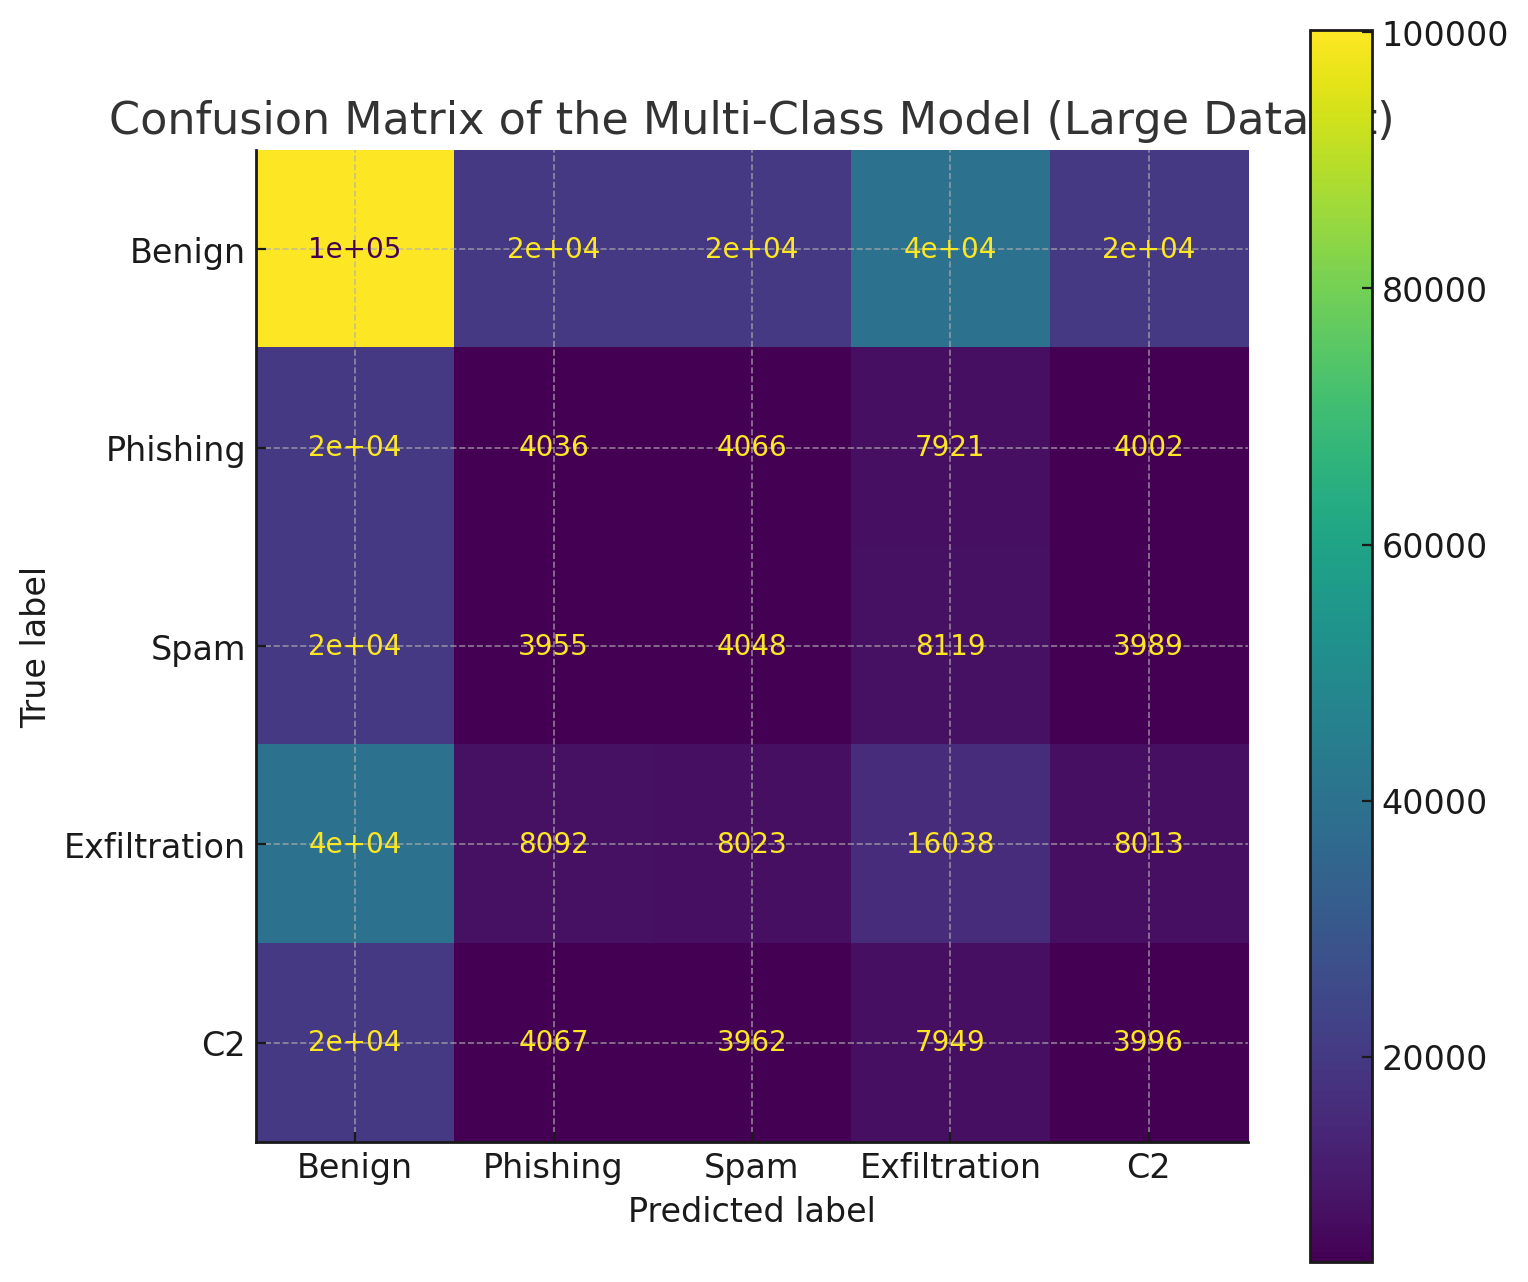
\includegraphics[width=1\linewidth]{Chap3//images/confusionMatrixmuliclass.png}
    \caption{Confusion Matrix of the Multi-Class Model}
    \label{}
\end{figure}
The diagonal cells of the matrix show the number of correctly classified instances for each class, while the off-diagonal cells indicate misclassifications. For example, the cell corresponding to the row labeled "Phishing" and the column labeled "Spam" represents the number of phishing instances that were incorrectly classified as spam. This matrix helps us understand the distribution of errors across different classes and highlights the model's ability to distinguish between benign traffic and various types of DNS-based attacks, including phishing, spamming, data exfiltration, and command and control (C2) communication.

\paragraph{Evaluation Metrics}
The evaluation metrics, including precision, recall, and F1-score, provide a comprehensive assessment of the model's performance for each class. These metrics are summarized in Table \ref{tab:evaluation_metrics}.

\begin{table}[h]
    \centering
    \caption{Precision, Recall, and F1-Score by Class}
    \label{tab:evaluation_metrics}
    \begin{tabular}{|l|c|c|c|}
        \hline
        \textbf{Class} & \textbf{Precision} & \textbf{Recall} & \textbf{F1-Score} \\
        \hline
        Benign & 0.93 & 0.94 & 0.93 \\
        Phishing & 0.94 & 0.93 & 0.92 \\
        Spam & 0.88 & 0.93 & 0.89 \\
        Exfiltration & 0.98 & 0.96 & 0.93 \\
        C2 & 0.94 & 0.96 & 0.92 \\
        \hline
    \end{tabular}
\end{table}

This table provides a clear overview of the model's precision, recall, and F1-score for each class, highlighting the model's strengths and areas for potential improvement. Precision indicates the proportion of true positive predictions among the predicted positives, recall measures the proportion of true positives among the actual positives, and F1-score represents the harmonic mean of precision and recall, offering a balanced measure of the model's performance.





In summary, the use of the Random Forest classifier, coupled with thorough evaluation metrics, allows us to develop a robust multi-class classification model. This model significantly enhances the detection and mitigation of various DNS-based attacks, thereby improving the overall security of network systems.




\mySection{Results and discussions}{}

\subsubsection{Performance metrics}
\subsubsection{Evaluation approach}
\subsubsection{Comparison with related work}
\mySection{Overall Comparison And Discussion}{}
\subsection{Comparison of binary and multiple classification results}
\mySection{Conclusion}{}